
\begin{frame}[fragile]

Map the input question to the most relevant normal form.
  
\onslide<2->{
\begin{center}
  \alert{Where does the prime minister of the United Kingdom live?}
\end{center}}

\begin{figure}
 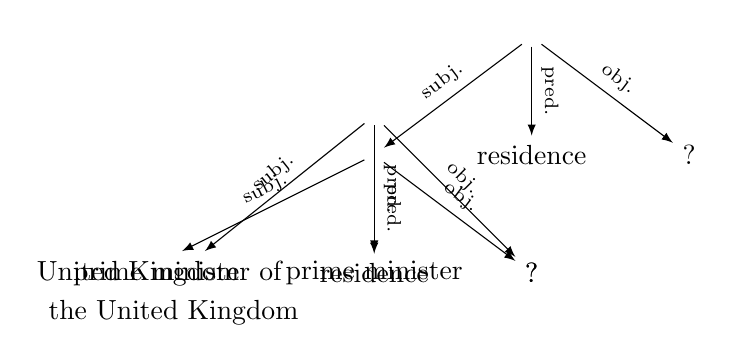
\begin{tikzpicture}
  \onslide<2>{
  \node (7) at (8,9) {$\triple$};
  \node (8) at (5.5,7) {prime minister of};
  \node (11) at (5.45,6.5) {the United Kingdom};
  \node (9) at (8,7) {residence};
  \node (10) at (10,7) {?};

  \draw[->, >=latex] (7) edge node[sloped, anchor=center, above] {\scriptsize{subj.}} (8);
  \draw[->, >=latex] (7) edge node[sloped, anchor=center, above] {\scriptsize{pred.}} (9);
  \draw[->, >=latex] (7) edge node[sloped, anchor=center, above] {\scriptsize{obj.}} (10);}
  
  \onslide<3>{  
  \node (0) at (10,10) {$\triple$};
  \node (1) at (10,8.5) {residence};
  \node (2) at (12,8.5) {?};
  \node (3) at (8,8.5) {$\triple$};
  \node (4) at (8,7) {prime minister};
  \node (5) at (5,7) {United Kingdom};
  \node (6) at (10,7) {?};

  \draw[->, >=latex] (0) edge node[sloped, anchor=center, above] {\scriptsize{obj.}} (2);
  \draw[->, >=latex] (0) edge node[sloped, anchor=center, above] {\scriptsize{pred.}} (1);
  \draw[->, >=latex] (0) edge node[sloped, anchor=center, above] {\scriptsize{subj.}} (3);
  \draw[->, >=latex] (3) edge node[sloped, anchor=center, above] {\scriptsize{subj.}} (5);
  \draw[->, >=latex] (3) edge node[sloped, anchor=center, above] {\scriptsize{obj.}} (6);
  \draw[->, >=latex] (3) edge node[sloped, anchor=center, above] {\scriptsize{pred.}} (4);}
 \end{tikzpicture}
\end{figure}

\end{frame}
